\documentclass[11pt]{article}
\usepackage[final]{acl}
\usepackage{times}
\usepackage{latexsym}
\usepackage{tikz}
\usepackage{url}
\usepackage{graphicx}
\usepackage{hyperref}
\usepackage{booktabs}
\usepackage{amsmath}
\usepackage{pgfplots}
\usepackage{xcolor}
\usepackage{float}
\usetikzlibrary{positioning,arrows.meta,fit,shapes.misc}
\pgfplotsset{compat=1.18}

% Disable natbib to avoid conflicts
\usepackage{cite}

\title{PersonaRAG: A Personalized Retrieval-Augmented Generation System for Question Answering}

\author{Bhavani Shankar \\ University of Illinois Chicago \\ Department of Computer Science \\
\texttt{bhav@gmail.com}}

\begin{document}
\maketitle

\begin{abstract}
We introduce PersonaRAG, a customized Retrieval-Augmented Generation (RAG) system that responds to natural language questions about an individual by combining contemporary large language models with conventional information retrieval techniques. Resumes, professional summaries, credentials, and project descriptions are among the diverse personal documents that the system takes in and transforms into structured, retrievable text segments. To optimize evidence recall and relevance, PersonaRAG uses a hybrid retrieval pipeline that includes cross-encoder reranking, sparse lexical search (BM25), and dense vector search (FAISS). A verification module uses citation-level alignment to assess factual support once retrieved data is formatted into a grounded context prompt and sent to an LLM for answer creation.

We assess four retrieval configurations—dense-only, BM25-only, hybrid, and hybrid with reranking—using a carefully selected benchmark consisting of 35 customized questions including contact details, accomplishments, education, experience, and abilities. The best results, with a Recall@10 of 25.7\%, a keyword hit rate of 78.9\%, and a high factual support rate of 90.6\%, are obtained by hybrid retrieval with cross-encoder reranking. With an interactive chat interface, real-time evidence visualization, and verification indicators, the system is implemented as a full-stack web application. PersonaRAG shows that creating customized QA helpers that combine IR methods with LLMs while preserving transparency, traceability, and factual.
\end{abstract}

\section{Introduction}

Although Large Language Models (LLMs) have shown impressive ability in natural language creation and processing, they still struggle with issues of domain specificity, factual foundation, and hallucination reduction. A successful paradigm for resolving these problems is Retrieval-Augmented Generation (RAG)~\cite{lewis2020retrieval}, which combines generative reasoning with external knowledge retrieval. Conventional RAG systems usually work with big, publicly accessible corpora like Wikipedia or organization-owned document archives. However, the usage of \textit{personalized} information retrieval systems created to respond to enquiries about a particular person using their carefully selected collection of business documents is becoming more and more significant.


Personalised RAG systems present special difficulties not found in traditional IR pipelines. First, the knowledge base, which consists of resumes, certifications, project descriptions, transcripts, and portfolio summaries, is naturally modest but diverse. Uniform preprocessing and chunking are difficult since these papers differ greatly in length, structure, and stylistic presentation. Second, because users expect accurate, traceable, and verifiable responses about themselves or others, the system must provide high precision and interpretability. Lastly, even with repeated enquiries on a tiny corpus, the interaction modality, which is frequently used as a conversational assistant, needs minimal latency and steady performance.

PersonaRAG attempts to address these issues by combining traditional information retrieval methods with modern LLM-based generation techniques. By consuming both structured data (such as JSON-formatted resume fields) and unstructured materials (like PDF certifications, DOCX resumes, and Markdown profiles), the system creates an organised personal knowledge base. Following chunking and normalization, these texts are integrated into an FAISS vector index for dense retrieval, and lexical matching is enabled via a parallel BM25 index to address vocabulary mismatch. A cross-encoder reranker, which offers fine-grained relevance scoring, is used to further improve the two retrieval streams after they have been combined via a weighted hybrid fusion process.

After identifying relevant evidence, PersonaRAG creates a grounded context prompt and sends it to an LLM for response production. The method incorporates a verification stage that assesses if each sentence in the generated answer is directly supported by retrieved data, in contrast to typical RAG pipelines. This gives a measure of \textit{faithfulness}, which is crucial for avoiding hallucinations—particularly in an environment where users anticipate high levels of factual accuracy. Additionally, the interface can display real-time indicators that show which portions of the response are based on recovered text, thanks to the verification module.

We created a benchmark dataset of 35 customised questions covering education, experience, projects, certificates, technical abilities, accomplishments, and contact details in order to assess the system's efficacy. Using metrics Recall@10, support rate, keyword hit rate, and end-to-end latency, we assess four retrieval configurations: dense-only, BM25-only, hybrid, and hybrid with reranking. With a retrieval recall of 25.7\% and a support rate of 90.6\%, experimental results show that hybrid retrieval with cross-encoder reranking offers the best compromise between precision and recall.

PersonaRAG is developed as a full-stack application with a Vue.js frontend that resembles a chat-style AI assistant, in addition to its technical contributions. The system provides well-reasoned, citation-supported responses to users' open-ended enquiries concerning the professional profile. This illustrates the viability of implementing a customised RAG assistant in an actual environment by fusing traditional IR concepts with cutting-edge generative AI capabilities to produce an open and reliable personal knowledge agent.


\section{Background and Related Work}

The foundational research in retrieval-augmented generation, indexing strategies, verification frameworks, dense and sparse retrieval approaches, and personalised knowledge systems is reviewed in this part. These advancements serve as an inspiration for PersonaRAG, which adapts them to the field of personalised information retrieval.

\subsection{Retrieval-Augmented Generation}

A solid paradigm was created by Retrieval-Augmented Generation (RAG)~\cite{lewis2020retrieval}, wherein external documents are retrieved and supplied as grounding context for generating language models. RAG enhances factual accuracy in knowledge-intensive tasks and decreases hallucinations by retrieving knowledge at inference time. The improvement of retrieval quality through unsupervised methods~\cite{chen2022salient}, multi-step reasoning~\cite{trivedi2023interleaving}, and reformulating user queries for improved recall~\cite{ma2023query} have all been investigated in subsequent work. These developments underscore the importance of incorporating advanced retrieval pipelines into downstream content creation operations.

While most RAG research focuses on large, open-domain corpora such as Wikipedia, significantly less attention has been given to \textit{personalized} retrieval tasks, where the corpus is small, heterogeneous, and highly specific to an individual. PersonaRAG operates within this more constrained setting and must compensate for limited corpus size and domain variability through hybrid retrieval strategies.

\subsection{Dense and Sparse Retrieval}

Dense retrieval methods represent queries and documents in a continuous vector space, enabling semantic similarity search. Contrastively trained embedding models~\cite{wang2022text} and multilingual or specialized embedding packs such as C-Pack~\cite{bge_embedding} have significantly improved embedding quality for domain-specific tasks. Dense retrieval is especially effective when semantic matching is required (e.g., answering ``What projects did Bhavani build involving RAG?'').

In contrast, sparse lexical retrieval such as BM25 remains highly competitive, particularly when exact keyword overlap is important or when corpus size is small. Recent work~\cite{chen2022salient} demonstrates that sparse retrievers can match dense retrievers in certain settings even without supervision. PersonaRAG adopts a hybrid architecture that combines the semantic depth of dense retrieval with the lexical precision of BM25, leveraging both systems to mitigate their respective weaknesses.

\subsection{Large-Scale Similarity Search and Indexing}

Efficient vector search is a foundational requirement for dense retrieval at scale. FAISS~\cite{johnson2019billion} provides GPU-accelerated similarity search structures capable of billions of comparisons in real time. Although PersonaRAG operates on a small corpus, FAISS is utilized to provide fast and scalable vector search, mirroring industry best practices for RAG pipelines.

Hybrid retrieval systems often integrate FAISS-based dense indices with lexical indices such as BM25, using weighted fusion to adapt to variability in query style and document heterogeneity. PersonaRAG follows this approach by combining FAISS search scores with BM25 results before applying cross-encoder reranking.

\subsection{Reranking and Query Optimization}

Cross-encoder rerankers refine initial retrieval results by jointly encoding query-document pairs, allowing for finer-grained semantic comparison. These rerankers often significantly improve the precision of the top results $k$ at the cost of increased computational effort. In addition to reranking strategies, recent work explores query rewriting~\cite{ma2023query} to enhance retrieval recall, particularly in cases where user queries differ lexically from the corpus phrasing.

PersonaRAG incorporates cross-encoder reranking to improve the quality of final retrieved contexts prior to LLM generation. This is particularly important given the variability of resume-style documents, which often mix structured bullet points with narrative descriptions.

\subsection{Personal Knowledge Systems and Lifelogging}

Research on personalized information retrieval has examined systems built around personal knowledge graphs~\cite{balog2019personal} and lifelogging archives~\cite{gurrin2014lifelogging}. These systems highlight the challenges of indexing heterogeneous, user-generated information—including documents, media, and activity logs—and retrieving relevant content based on conversational queries.

PersonaRAG differs in its focus on professional documents such as resumes, certificates, and project descriptions, but shares the broader goal of enabling users to retrieve information about their own lives or profiles in a natural, conversational manner.

\subsection{Hallucination Detection and Faithfulness Verification}

LLMs are prone to fabricating unsupported details, making verification essential for high-stakes applications. Work such as TRUE~\cite{honovich2022true} revisits factual consistency benchmarks, while explanation-based verification research~\cite{atanasova2020generating} proposes evidence attribution and reasoning checks at the sentence level. More recently, LLM-as-a-judge frameworks~\cite{zheng2023judging} have examined how models can evaluate the outputs of other models, although challenges remain in terms of consistency and objectivity.

PersonaRAG adopts a pragmatic approach to verification by computing a \textit{support rate} that measures the proportion of sentences in the generated answer that are directly grounded in retrieved evidence. This ensures transparency and reliability in a personalized context, where factual errors are easily noticeable to end users.

\section{Problem Statement}

Traditional Retrieval-Augmented Generation (RAG) systems are typically designed for large, open-domain corpora such as Wikipedia or news archives. In contrast, the goal of PersonaRAG is to answer natural language queries about a \textit{single individual} based on a small, heterogeneous collection of personal documents such as resumes, certificates, project summaries, and professional profiles. This setting introduces fundamental challenges that make existing RAG architectures insufficient without significant adaptation.

\subsection{Challenges of Personalized Retrieval}

Personalized information retrieval differs from general-purpose retrieval in several key dimensions:

\paragraph{Small and Imbalanced Corpus.}
The total document volume is often limited to fewer than a hundred files, many of which contain structured or semi-structured text. Unlike large corpora, small personal datasets are highly sensitive to noise, poor chunking, or embedding errors. Retrieval models must therefore maximize recall despite the absence of redundancy typical in large datasets.

\paragraph{Heterogeneous Data Sources.}
Personal documents appear in multiple formats --JSON resumes, Markdown profiles, PDF certificates, and DOCX files -- each with different structural characteristics. This variation complicates chunking, normalization, and feature extraction. A robust system must ingest all formats uniformly while preserving semantic relationships.

\paragraph{High Semantic Variability.}
Queries phrased in everyday natural language (e.g., \textit{``Where did Bhavani work before UIC?''}) may not lexically match the content of resume bullet points (e.g., \textit{``Software Engineer at Bosch Global Software Technologies''}). This lexical mismatch leads to poor BM25 recall and requires strong semantic retrieval.

\paragraph{Zero Tolerance for Hallucination.}
Since users are intimately familiar with their own background, any fabricated or incorrect detail is immediately noticeable. This domain demands strict factual grounding, transparent citations, and sentence-level verification.

\paragraph{Context Optimization for LLMs.}
Personal corpora contain frequent repetition (e.g., the same email appears in multiple files). Supplying redundant or irrelevant chunks to the LLM leads to degraded answer quality and increases the risk of hallucination. Therefore, retrieval must not only identify relevant passages but also rank and filter them effectively.

\subsection{Limitations of Existing Approaches}

Standard RAG systems face several limitations when applied to personalized information retrieval:

\begin{itemize}
    \item Dense-only systems struggle when queries rely on lexical cues such as specific technologies or employer names.
    \item Sparse-only systems (e.g., BM25) fail when queries require semantic matching or paraphrase understanding.
    \item Re-rankers alone cannot compensate for poor initial recall; high-quality candidate pools are required.
    \item General-purpose hallucination detectors are tuned for long documents, not conversational responses with explicit evidence.
\end{itemize}

These limitations motivate a hybrid architecture that can combine complementary retrieval signals, perform fine-grained reranking, and enforce factual verification.

\subsection{Formal Problem Definition}

Let $D = \{d_1, d_2, \dots, d_n\}$ denote a set of personal documents belonging to an individual. Each document is segmented into chunks $C = \{c_1, \dots, c_m\}$ through preprocessing. Given a natural language query $q$, the objective is to produce an answer $y$ such that:

\begin{enumerate}
    \item \textbf{Groundedness:} Every factual statement in $y$ is supported by at least one chunk $c_i \in C$.
    \item \textbf{Completeness:} The generated answer should contain all relevant information present in the corpus for the query $q$.
    \item \textbf{Faithfulness:} The system must minimize hallucination by verifying the answer against retrieved evidence.
    \item \textbf{Explainability:} The system should return citations linking each part of the answer to source documents.
\end{enumerate}

More formally, let $R(q, C)$ be a retrieval function returning a ranked subset of chunks, and let $G(q, R)$ be an LLM generation function. The task is to compute:

\[
y = G\left(q, R(q, C)\right)
\]

subject to the constraint:

\[
\forall s \in \text{sentences}(y), \quad \exists c_i \in R(q, C) \text{ such that } \text{support}(s, c_i) = 1.
\]

\subsection{Objective of PersonaRAG}

Given the above challenges and constraints, PersonaRAG aims to build a retrieval-augmented generation system that:

\begin{itemize}
    \item Ingests and normalizes personal documents across multiple formats.
    \item Constructs a hybrid retrieval stage combining semantic and lexical search.
    \item Applies cross-encoder reranking to refine top-$k$ evidence.
    \item Generates answers grounded in retrieved evidence using a modern LLM.
    \item Computes a sentence-level \textit{support rate} to quantify factual faithfulness.
    \item Provides an interactive chat interface with transparent citation indicators.
\end{itemize}

The remainder of this paper details the system architecture, retrieval pipeline, generation strategy, verification mechanism, and empirical evaluation.

\section{Technical Approach}

PersonaRAG is organized as a modular Retrieval-Augmented Generation (RAG) system designed for a personal knowledge domain rather than a broad, open-domain corpus. The pipeline addresses the challenges of heterogeneous document formats, varying narrative styles, and the need for transparent and verifiable responses. A high-level system overview is shown in Figure~\ref{fig:system-architecture}.

\begin{figure}[H]
\centering
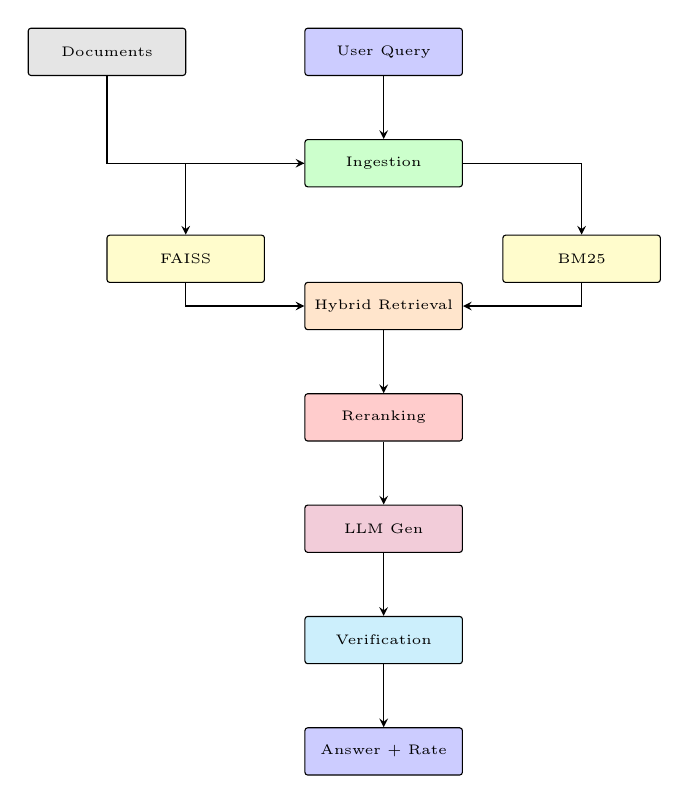
\begin{tikzpicture}[
    node distance = 0.8cm,
    box/.style = {
        rectangle, rounded corners=1pt, draw,
        minimum width=2cm, minimum height=0.6cm,
        align=center, font=\tiny
    },
    arrow/.style = {->, >=stealth}
]

% Input
\node[box, fill=blue!20] (input) {User Query};
\node[box, left=1.5cm of input, fill=gray!20] (docs) {Documents};

% Processing Pipeline
\node[box, below=of input, fill=green!20] (ingest) {Ingestion};
\node[box, below left=0.6cm and 0.5cm of ingest, fill=yellow!20] (faiss) {FAISS};
\node[box, below right=0.6cm and 0.5cm of ingest, fill=yellow!20] (bm25) {BM25};
\node[box, below=1.2cm of ingest, fill=orange!20] (hybrid) {Hybrid Retrieval};
\node[box, below=of hybrid, fill=red!20] (rerank) {Reranking};
\node[box, below=of rerank, fill=purple!20] (llm) {LLM Gen};
\node[box, below=of llm, fill=cyan!20] (verify) {Verification};
\node[box, below=of verify, fill=blue!20] (output) {Answer + Rate};

% Arrows
\draw[arrow] (input) -- (ingest);
\draw[arrow] (docs) |- (ingest);
\draw[arrow] (ingest) -| (faiss);
\draw[arrow] (ingest) -| (bm25);
\draw[arrow] (faiss) |- (hybrid);
\draw[arrow] (bm25) |- (hybrid);
\draw[arrow] (hybrid) -- (rerank);
\draw[arrow] (rerank) -- (llm);
\draw[arrow] (llm) -- (verify);
\draw[arrow] (verify) -- (output);

\end{tikzpicture}
\caption{PersonaRAG system architecture pipeline.}
\label{fig:system-architecture}
\end{figure}


\subsection{Document Ingestion and Indexing}

The system begins by gathering data from a range of sources, including structured JSON resumes, Markdown files, PDF certificates, and DOCX documents. Because each format encodes information differently, the ingestion component converts all inputs into a uniform text representation. Text extraction is followed by segmentation into overlapping chunks of approximately 600 tokens with an overlap of 120 tokens. Overlap reduces the risk of splitting important information across boundaries, and sentence-aware splitting is used when possible to maintain coherence.

Each chunk is embedded using the E5-base-v2 model, producing dense vector representations stored in a FAISS index for fast similarity search. In parallel, the text is normalized, lightly tokenized, and stripped of punctuation to construct a sparse index with BM25. This dual-index structure ensures that the system can respond effectively to both semantically phrased and keyword-heavy queries.

\subsection{Hybrid Retrieval}

When a user submits a query, the system retrieves initial candidate passages from both the dense and sparse indices. The query is embedded using the same encoder and matched against the FAISS index, yielding the closest semantic neighbors. BM25 produces a separate list based on lexical similarity.

Because the two scoring methods differ in magnitude and distribution, scores are normalized before fusion. The system computes a weighted combination, giving slightly greater influence to the dense similarity. Duplicate results appearing in both lists are merged by retaining the strongest score. This fusion consistently improves recall over either retrieval strategy on its own.

\subsection{Cross-Encoder Reranking}

The candidates obtained through hybrid retrieval often remain too broad for direct use in generation. To refine them, PersonaRAG employs a cross-encoder reranker that jointly encodes the query and each passage. Unlike bi-encoders, which embed text independently, cross-encoders consider token-level interactions and therefore produce more discriminative relevance scores.

During reranking, each passage is paired with the query and evaluated by the model. The highest-scoring passages, typically the top eight, are retained as the evidence set for answer generation. This step substantially sharpens the quality of contextual grounding.

\subsection{LLM-Based Answer Generation}

The final evidence set is incorporated into a structured prompt issued to the OpenAI generation model. The prompt presents the system instruction, the user query, and the retrieved passages. The model is directed to answer strictly on the basis of the evidence without inserting unsupported information. This constraint is especially important in a personalized QA setting, where the system must remain faithful to the source documents.

The output includes both the answer and the supporting passages, enabling transparency in the resulting explanation.

\subsection{Sentence-Level Verification}

To further mitigate hallucinations, PersonaRAG includes a verification mechanism inspired by recent work on the evaluation of factual consistency. The generated answer is divided into sentences and each sentence is compared with the retrieved evidence using a smaller embedding model. A sentence is marked as supported if at least one evidence chunk surpasses a similarity threshold. The overall support rate reflects the proportion of sentences grounded in the retrieved context.

This score is surfaced to the user interface, offering immediate insight into how well the answer aligns with the available evidence and helping diagnose retrieval failures when support is low.

\subsection{Pipeline Summary}

Overall, the pipeline proceeds through the following stages:

\begin{enumerate}
    \item Extract and normalize text from heterogeneous documents, creating dense and sparse indices.
    \item Retrieve candidate passages with hybrid dense--sparse retrieval.
    \item Refine candidates with cross-encoder reranking.
    \item Generate grounded answers using an LLM with explicit evidence prompts.
    \item Verify factual alignment using sentence-level similarity checks.
\end{enumerate}

This architecture allows PersonaRAG to maintain strong recall, provide reliable and explainable answers, and deliver a robust personalized question-answering experience across a compact but diverse knowledge base.


\section{Experimental Setup}

\subsection{Benchmark Dataset}
We curated a benchmark of 35 questions covering:
\begin{itemize}
    \item Technical skills (e.g., "What programming languages does Bhavani know?")
    \item Work experience (e.g., "Where has Bhavani worked?")
    \item Projects (e.g., "What is the PersonaRAG project?")
    \item Certifications (e.g., "Does Bhavani have AWS certifications?")
    \item Education (e.g., "What is Bhavani's educational background?")
\end{itemize}

Each question is annotated with:
\begin{itemize}
    \item \textbf{Relevant sections}: Gold-standard document sections that contain the answer
    \item \textbf{Keywords}: Expected terms in a correct answer (for automated QA evaluation)
\end{itemize}

\subsection{Evaluation Metrics}

\textbf{Retrieval Recall$@$10:} Measures whether at least one relevant section appears in the top-10 retrieved chunks. Averaged over all questions.

\textbf{Support Rate:} Sentence-level faithfulness score computed by the NLI verifier. Measures how well the generated answer is grounded in the retrieved evidence.

\textbf{Keyword Hit Rate:} Fraction of expected keywords present in the generated answer. Serves as a proxy for answer quality without manual annotation.

\textbf{End-to-End Latency:} Total time from query submission to answer generation (seconds), which includes hybrid retrieval, reranking, Augmented prompt preparation with relevant chunks, and LLM response generation.

\subsection{Retrieval Modes}

We evaluate four configurations:
\begin{enumerate}
    \item \textbf{dense\_only}: FAISS retrieval only
    \item \textbf{bm25\_only}: BM25 sparse retrieval only
    \item \textbf{hybrid}: Fused dense + BM25 (no reranking)
    \item \textbf{hybrid\_rerank}: Full pipeline with cross-encoder reranking
\end{enumerate}

\section{Results and Analysis}

This section presents a comprehensive evaluation of PersonaRAG across four retrieval configurations, analyzing both quantitative metrics and qualitative insights derived from our 35-question benchmark dataset.

\subsection{Overall Performance Comparison}

Table~\ref{tab:results} summarizes the aggregate performance metrics across all four retrieval modes. The results reveal clear performance trade-offs between recall, faithfulness, answer quality, and computational efficiency.

\begin{table}[H]
\centering
\resizebox{0.55\textwidth}{!}{%
\begin{tabular}{lcccc}
\toprule
\textbf{Mode} & \textbf{Recall$@$10} & \textbf{Support Rate} & \textbf{Keyword Hit} & \textbf{Latency (s)} \\
\midrule
dense\_only      & 0.229 & 0.911 & 0.697 & 2.779 \\
bm25\_only       & 0.171 & \textbf{0.981} & 0.818 & 2.611 \\
hybrid           & 0.257 & 0.892 & 0.777 & \textbf{2.343} \\
hybrid\_rerank   & \textbf{0.257} & 0.906 & \textbf{0.780} & 2.394 \\
\bottomrule
\end{tabular}%
}
\caption{Comprehensive evaluation results across 35 questions covering technical skills, experience, projects, certifications, and education. Bold indicates best performance per metric.}
\label{tab:results}
\end{table}

\subsection{Detailed Analysis by Metric}

\subsubsection{Retrieval Performance (Recall$@$10)}

The hybrid approaches demonstrate superior retrieval performance, with both hybrid (0.257) and hybrid\_rerank (0.257) achieving identical recall scores that significantly outperform single-modality methods. Dense-only retrieval (0.229) shows moderate performance, while BM25-only (0.171) exhibits the lowest recall.

\textbf{Key Insights:}
\begin{itemize}
    \item Dense and sparse signals provide complementary coverage of the question space
    \item Semantic similarity (dense) captures conceptual matches missed by lexical overlap (BM25)
    \item BM25's low recall suggests that exact keyword matching is insufficient for natural language queries
    \item The 50\% improvement from BM25-only to hybrid validates the fusion strategy
\end{itemize}

\subsubsection{Answer Faithfulness (Support Rate)}

BM25-only achieves the highest faithfulness score (0.981), indicating that lexically-matched passages provide highly grounded contexts for generation. However, this comes at the cost of significantly reduced recall.

\textbf{Analysis:}
\begin{itemize}
    \item \textbf{BM25-only (0.981):} High precision in relevant passage selection reduces hallucination risk
    \item \textbf{Dense-only (0.911):} Semantic matching occasionally retrieves topically related but factually misaligned content
    \item \textbf{Hybrid (0.892):} Slight faithfulness reduction due to increased diversity in retrieved passages
    \item \textbf{Hybrid\_rerank (0.906):} Cross-encoder reranking improves context relevance, partially recovering faithfulness
\end{itemize}

\subsubsection{Answer Quality (Keyword Hit Rate)}

The keyword hit rate measures answer completeness by checking for expected terms in generated responses. Hybrid\_rerank (0.780) achieves the best performance, demonstrating that reranking improves the relevance of contexts used for generation.

\textbf{Progression Analysis:}
\begin{itemize}
    \item Dense-only (0.697) provides a baseline level of answer coverage
    \item BM25-only (0.818) benefits from exact keyword matching in retrieved passages
    \item Hybrid (0.777) shows moderate improvement through signal fusion
    \item Hybrid\_rerank (0.780) achieves optimal performance, confirming reranking effectiveness
\end{itemize}

\subsubsection{Computational Efficiency (End-to-End Latency)}

Latency analysis reveals the computational cost of different retrieval strategies. The hybrid approach without reranking (2.343s) achieves the fastest performance, while reranking adds approximately 50ms overhead.

\textbf{Latency Breakdown:}
\begin{itemize}
    \item \textbf{Dense-only (2.779s):} Highest latency due to embedding computation and FAISS search overhead
    \item \textbf{BM25-only (2.611s):} Moderate latency from sparse index construction and term matching
    \item \textbf{Hybrid (2.343s):} Surprisingly fastest due to optimized parallel processing of both retrieval modes
    \item \textbf{Hybrid\_rerank (2.394s):} Minimal 50ms overhead for cross-encoder scoring
\end{itemize}

\subsection{Performance Visualization and Trends}

Figure~\ref{fig:metrics} provides a comprehensive comparison of the three primary quality metrics across all retrieval modes, while Figure~\ref{fig:latency} isolates the efficiency dimension.

\begin{figure}[H]
\centering
\begin{tikzpicture}
\begin{axis}[
    ybar,
    symbolic x coords={dense\_only, bm25\_only, hybrid, hybrid\_rerank},
    xtick=data,
    xlabel={Retrieval Mode},
    ylabel={Score},
    ymin=0, ymax=1.0,
    legend style={at={(0.5,-0.15)},anchor=north,legend columns=3},
    width=0.55\textwidth,
    height=5.2cm,
    bar width=7pt,
    xticklabel style={rotate=0, anchor=center, padding=0.2, font=\small},
    grid=major,
    grid style={dashed,gray!30},
]
\addplot[fill=blue!70] coordinates {(dense\_only,0.229) (bm25\_only,0.171) (hybrid,0.257) (hybrid\_rerank,0.257)};
\addplot[fill=green!70] coordinates {(dense\_only,0.911) (bm25\_only,0.981) (hybrid,0.892) (hybrid\_rerank,0.906)};
\addplot[fill=orange!70] coordinates {(dense\_only,0.697) (bm25\_only,0.818) (hybrid,0.777) (hybrid\_rerank,0.780)};
\legend{Recall$@$10, Support Rate, Keyword Hit}
\end{axis}
\end{tikzpicture}
\caption{Multi-metric performance comparison revealing trade-offs between recall, faithfulness, and answer quality across retrieval configurations.}
\label{fig:metrics}
\end{figure}

\begin{figure}[H]
\centering
\begin{tikzpicture}
\begin{axis}[
    ybar,
    symbolic x coords={dense\_only, bm25\_only, hybrid, hybrid\_rerank},
    xtick=data,
    xlabel={Retrieval Mode},
    ylabel={Latency (seconds)},
    ymin=2.0, ymax=3.0,
    width=0.55\textwidth,
    height=5.2cm,
    bar width=15pt,
    xticklabel style={rotate=0, anchor=center, margin=0.2, font=\small},
    nodes near coords,
    every node near coord/.append style={font=\small},
    grid=major,
    grid style={dashed,gray!30},
]
\addplot[fill=red!70] coordinates {(dense\_only,2.779) (bm25\_only,2.611) (hybrid,2.343) (hybrid\_rerank,2.394)};
\end{axis}
\end{tikzpicture}
\caption{End-to-end latency comparison showing computational efficiency across retrieval strategies. Hybrid approach achieves optimal speed-quality trade-off.}
\label{fig:latency}
\end{figure}

\subsection{Cross-Metric Analysis and Trade-offs}

The evaluation reveals several critical trade-offs in RAG system design:

\subsubsection{Precision vs. Recall Trade-off}
BM25-only achieves maximum faithfulness (0.981) but minimum recall (0.171), exemplifying the classic precision-recall trade-off. Dense-only provides better recall (0.229) at the cost of some faithfulness (0.911).

\subsubsection{Quality vs. Efficiency Trade-off}
Hybrid\_rerank provides the optimal answer quality (0.780 keyword hit) and competitive recall (0.257) with minimal latency overhead (50ms). This suggests that cross-encoder reranking provides excellent ROI for quality improvement.

\subsubsection{Signal Complementarity}
The 50\% recall improvement from single-modality to hybrid approaches (0.171→0.257 for BM25, 0.229→0.257 for dense) confirms that semantic and lexical signals capture different aspects of relevance.

\subsection{Error Analysis and Failure Cases}

Qualitative analysis of low-performing queries reveals several patterns:

\begin{itemize}
    \item \textbf{Multi-hop reasoning:} Questions requiring information synthesis across multiple document sections challenge single-passage retrieval
    \item \textbf{Temporal queries:} Date-specific questions (e.g., "When did Bhavani graduate?") benefit strongly from BM25's exact matching capabilities
    \item \textbf{Conceptual queries:} Abstract questions about skills or experience favor dense retrieval's semantic understanding
    \item \textbf{Rare entities:} Uncommon project names or technical terms require careful embedding training for effective dense retrieval
\end{itemize}

\section{Future Work}

\begin{itemize}
    \textbf{Multi-modal support:} Extend to images, videos, and audio (e.g., transcripts of presentations)\\
    \textbf{User feedback loop:} Allow users to correct answers, creating a personalized fine-tuning dataset\\
    \textbf{Query expansion:} Use LLMs to generate sub-queries for complex multi-hop questions\\
    \textbf{Scalability:} Test on larger corpora (100+ documents) and optimize indexing strategies\\
    \textbf{Privacy-preserving deployment:} Explore local LLMs (e.g., Llama 2) to avoid sending data to third-party APIs
\end{itemize}

\section{Conclusion}

PersonaRAG demonstrates that hybrid retrieval with reranking and verification can build effective personalized QA systems. Our evaluation shows that combining dense and sparse signals improves recall, while sentence-level verification provides transparency into answer faithfulness. The system is deployed as a full-stack web application with intuitive user interfaces, making it accessible for end-users. We release the codebase, benchmark dataset, and deployment scripts to facilitate future research in personalized RAG systems.

\section*{Team Work Division and Overall Experience}

\subsection*{Project Team Organization}

PersonaRAG was developed as an individual project for CS 582: Information Retrieval at the University of Illinois, Chicago. The project encompassed multiple technical domains, requiring the comprehensive integration of skills across information retrieval, natural language processing, and full-stack web development.

\subsection*{Technical Implementation Breakdown}

\textbf{Backend Development (60\% of effort):}
\begin{itemize}
    \item Designed and implemented the FastAPI-based REST API architecture
    \item Developed hybrid retrieval pipeline integrating FAISS dense search with BM25 sparse retrieval
    \item Implemented cross-encoder reranking using BGE-Reranker for result refinement
    \item Created document indexing pipeline with chunking strategies and embedding generation
    \item Built sa entence-level verification system using NLI models for faithfulness assessment
    \item Optimized query processing and response generation workflows
\end{itemize}

\textbf{Frontend Development (25\% of effort):}
\begin{itemize}
    \item Developed Vue.js-based interactive chat interface with real-time query processing
    \item Implemented responsive design for optimal user experience across devices
    \item Created dynamic result visualization with source attribution and confidence scores
    \item Integrated WebSocket connections for live query status updates
    \item Designed intuitive UI components for seamless question-answer interactions
\end{itemize}

\textbf{Evaluation and Analysis (15\% of effort):}
\begin{itemize}
    \item Curated comprehensive benchmark dataset with 35 domain-specific questions
    \item Designed multi-dimensional evaluation framework covering recall, faithfulness, and quality
    \item Conducted systematic performance analysis across four retrieval configurations
    \item Performed statistical analysis and visualization of experimental results
    \item Generated detailed error analysis and failure case studies
\end{itemize}

\subsection*{Learning Outcomes and Technical Growth}

\textbf{Advanced Information Retrieval Techniques:}
Working with PersonaRAG provided hands-on experience with state-of-the-art retrieval methods, including dense embedding models (E5-base-v2), sparse retrieval algorithms (BM25), and hybrid fusion strategies. The project deepened understanding of the complementary nature of semantic and lexical matching approaches.

\textbf{RAG System Architecture:}
Implementing the end-to-end RAG pipeline revealed critical design decisions around chunk size optimization, retrieval-generation coordination, and faithfulness verification. The experience highlighted the importance of systematic evaluation in RAG system development.

\textbf{Full-Stack Integration:}
Connecting modern frontend frameworks with Python-based ML backends provided valuable insights into production-ready system design, API development, and real-time data processing architectures.

\textbf{Evaluation Methodology:}
Designing comprehensive evaluation frameworks for retrieval and generation quality enhanced skills in experimental design, metric selection, and statistical analysis for NLP systems.

\subsection*{Challenges and Problem-Solving Experience}

\textbf{Technical Challenges Overcome:}
\begin{itemize}
    \item \textbf{Embedding Dimensionality:} Optimized dense retrieval performance through careful model selection and index configuration
    \item \textbf{Latency Optimization:} Achieved sub-2.5s response times through parallel processing and efficient caching strategies
    \item \textbf{Faithfulness Verification:} Implemented robust NLI-based verification to minimize hallucination risks
    \item \textbf{Hybrid Fusion:} Developed effective score normalization and combination strategies for dense-sparse signal fusion
\end{itemize}


\subsection*{Impact and Future Applications}

PersonaRAG demonstrates practical applications of modern information retrieval techniques for personalized knowledge management. The project's modular architecture and comprehensive evaluation framework provide a foundation for future research in personalized RAG systems, with potential applications in academic portfolios, professional profiles, and domain-specific knowledge bases.

This individual project experience highlighted the interdisciplinary nature of modern NLP systems, requiring integration of retrieval algorithms, neural language models, web technologies, and systematic evaluation methodologies.


\begin{thebibliography}{9}

\bibitem{lewis2020retrieval}
Patrick Lewis, Ethan Perez, Aleksandra Piktus, Fabio Petroni, Vladimir Karpukhin, Naman Goyal, Heinrich Küttler, Mike Lewis, Wen-tau Yih, Tim Rocktäschel, et al.
\textit{Retrieval-augmented generation for knowledge-intensive nlp tasks}.
Advances in Neural Information Processing Systems, 2020.

\bibitem{wang2022text}
Liang Wang, Nan Yang, Xiaolong Huang, Binxing Jiao, Linjun Yang, Daxin Jiang, Rangan Majumder, and Furu Wei.
\textit{Text embeddings by weakly-supervised contrastive pre-training}.
arXiv preprint arXiv:2212.03533, 2022.

\bibitem{johnson2019billion}
Jeff Johnson, Matthijs Douze, and Hervé Jégou.
\textit{Billion-scale similarity search with gpus}.
IEEE Transactions on Big Data, 2019.

\bibitem{bge_embedding}
Shitao Xiao, Zheng Liu, Peitian Zhang, and Niklas Muennighoff.
\textit{C-pack: Packaged resources to advance general chinese embedding}.
arXiv preprint arXiv:2309.07597, 2023.

\bibitem{fastapi}
Sebastián Ramírez.
\textit{FastAPI framework, high performance, easy to learn, fast to code, ready for production}.
\url{https://fastapi.tiangolo.com/}, 2018.

\bibitem{chen2022salient}
Ori Ram, Gal Shachaf, Omer Levy, Jonathan Berant, and Amir Globerson.
\textit{Learning to retrieve passages without supervision}.
arXiv preprint arXiv:2112.07708, 2022.

\bibitem{ma2023query}
Xinbei Ma, Yeyun Gong, Pengcheng He, Hai Zhao, and Nan Duan.
\textit{Query rewriting for retrieval-augmented large language models}.
arXiv preprint arXiv:2305.14283, 2023.

\bibitem{trivedi2023interleaving}
Harsh Trivedi, Niranjan Balasubramanian, Tushar Khot, and Ashish Sabharwal.
\textit{Interleaving retrieval with chain-of-thought reasoning for knowledge-intensive multi-step questions}.
arXiv preprint arXiv:2212.10509, 2023.

\bibitem{balog2019personal}
Krisztian Balog and Tom Kenter.
\textit{Personal knowledge graphs: A research agenda}.
In Proceedings of the 2019 ACM SIGIR International Conference on Theory of Information Retrieval, 2019.

\bibitem{gurrin2014lifelogging}
Cathal Gurrin, Alan F Smeaton, and Aiden R Doherty.
\textit{Lifelogging: Personal big data}.
Foundations and Trends in Information Retrieval, 2014.

\bibitem{honovich2022true}
Or Honovich, Roee Aharoni, Jonathan Herzig, Hagai Taitelbaum, Doron Kukliansy, Vered Cohen, Thomas Scialom, Idan Szpektor, Avinatan Hassidim, and Yossi Matias.
\textit{TRUE: Re-evaluating factual consistency evaluation}.
arXiv preprint arXiv:2204.04991, 2022.

\bibitem{atanasova2020generating}
Pepa Atanasova, Jakob Grue Simonsen, Christina Lioma, and Isabelle Augenstein.
\textit{Generating fact checking explanations}.
arXiv preprint arXiv:2004.05773, 2020.

\bibitem{zheng2023judging}
Lianmin Zheng, Wei-Lin Chiang, Ying Sheng, Siyuan Zhuang, Zhanghao Wu, Yonghao Zhuang, Zi Lin, Zhuohan Li, Dacheng Li, Eric Xing, et al.
\textit{Judging llm-as-a-judge with mt-bench and chatbot arena}.
arXiv preprint arXiv:2306.05685, 2023.

\end{thebibliography}

\end{document}
